% =============================================================================
%  TVC MPC Report — SC421 Model Predictive Control Project
%  Compile with:  pdflatex tvc_mpc_report.tex  (run twice for references)
% =============================================================================
\documentclass[11pt,a4paper]{article}

\usepackage[a4paper, top=2.4cm, bottom=2.4cm, left=2.5cm, right=2.5cm]{geometry}
\usepackage{amsmath, amssymb, bm}
\usepackage{amsthm}
\newtheorem{theorem}{Theorem}
\usepackage{booktabs}
\usepackage{graphicx}
\usepackage{subcaption}
\usepackage{hyperref}
\usepackage[numbers, sort&compress]{natbib}
\usepackage{xcolor}
\usepackage{enumitem}
\usepackage{parskip}
\usepackage{siunitx}     % \SI{5}{\degree}, \si{\radian} etc.
\usepackage{textcomp}    % \textdegree fallback

% Degree shorthand in math mode
\newcommand{\degree}{^\circ}

% Compact section spacing
\usepackage{titlesec}
\titlespacing*{\section}{0pt}{8pt}{4pt}
\titlespacing*{\subsection}{0pt}{6pt}{2pt}

% Math macros
\newcommand{\vect}[1]{\bm{#1}}
\newcommand{\mat}[1]{\mathbf{#1}}
\newcommand{\R}{\mathbb{R}}
\newcommand{\N}{\mathbb{N}}
\newcommand{\eset}{\mathcal{X}}
\newcommand{\uset}{\mathcal{U}}
\newcommand{\xf}{\mathcal{X}_f}
\newcommand{\norm}[1]{\left\lVert #1 \right\rVert}

\title{\textbf{Thrust-Vector Control of a Rocket via Model Predictive Control}\\
       \large SC421 — Model Predictive Control (25)}
\author{[Student Name]}
\date{\today}

% =============================================================================
\begin{document}
\maketitle
\vspace{-4mm}

% =============================================================================
\section*{Abstract}
% =============================================================================
This report presents the design, analysis, and simulation of a Model Predictive
Controller (MPC) for a thrust-vector-controlled (TVC) rocket ascending vertically.
The six-state linearised model captures coupled lateral/pitch dynamics driven by
a gimballed engine.  Terminal ingredients---a Lyapunov terminal cost obtained from
the discrete algebraic Riccati equation (DARE) and a maximal LQR-invariant terminal
set---provide closed-loop stability and recursive feasibility guarantees.
A steady-state Kalman filter (discrete LQE) is paired with the MPC to handle
realistic sensor noise from GPS, IMU, and rate gyroscopes.
Numerical simulations on the nonlinear plant demonstrate constraint satisfaction,
disturbance rejection, robust observer-based state estimation, and superior
performance relative to a saturating LQR baseline.  The sensitivity of the
controller to prediction horizon length and cost-function weights is also
characterised.

% =============================================================================
\section{Introduction}
% =============================================================================

\subsection{Application Description}

Thrust vector control is the primary attitude-control mechanism of liquid-fuelled
launch vehicles and landers.  By gimballing the main engine, TVC simultaneously
generates a lateral force and a corrective torque about the centre of gravity (CG),
enabling full attitude and trajectory control without separate cold-gas thrusters.
The flight-mechanics analogy is an \emph{inverted pendulum mounted on a cart}: the
rocket's attitude is inherently unstable under aerodynamic disturbances, and the
gimbal is the only actuator coupling the translational and rotational channels
\cite{Wie1998, Greensite1970}.

\textbf{Why constraints matter.}
The gimbal actuator has a hard mechanical travel limit (here $|\delta| \leq 5^{\circ}$)
beyond which the nozzle may collide with the nozzle fairing.
Structural loads limit the allowable pitch angle ($|\theta| \leq 15^{\circ}$) to keep the
linearised model valid and prevent aerodynamic overload.  Thrust deviations
($|\Delta T| \leq 150\ \text{N}$) are bounded by the propellant feed system.

\textbf{Why MPC over LQR/PID.}
Classical LQR ignores actuator limits: at the initial pitch offset the unconstrained
gain saturates the gimbal, leading to overshoot and potential constraint violation.
PID cannot easily handle multivariable coupling (a single gimbal simultaneously
affects lateral and pitch dynamics).  MPC \emph{explicitly} enforces all constraints
at every prediction step, optimises over the full horizon, and provides verifiable
stability guarantees through terminal ingredients \cite{Mayne2000, RawlingsMayne2017}.

% ----- 1.2 ------------------------------------------------------------------
\subsection{System Model}

\textbf{Physical setup.}
A 50 kg sounding rocket ascends at a nominal climb speed $v_{z,\mathrm{nom}} =
15\ \mathrm{m/s}$ in the lateral--vertical $(y,z)$ plane (Fig.~\ref{fig:schematic}).
The main engine exerts nominal thrust $T_0 = mg = 490.5\ \mathrm{N}$.  The gimbal
is located $l_{\mathrm{tvc}} = 1.3\ \mathrm{m}$ below the CG; the moment of
inertia about the CG is $J = 80\ \mathrm{kg\cdot m^2}$.

\textbf{Nonlinear equations of motion.}  From Newton--Euler dynamics in the world
frame \cite{Wie1998}:
\begin{align}
  m\ddot{y}        &= (T_0+\Delta T)\sin(\theta+\delta),  \label{eq:nl_y} \\
  m\ddot{z}        &= (T_0+\Delta T)\cos(\theta+\delta) - mg, \label{eq:nl_z} \\
  J\ddot{\theta}   &= (T_0+\Delta T)\,l_{\mathrm{tvc}}\sin(\delta), \label{eq:nl_th}
\end{align}
where $\theta$ is the pitch angle from vertical (positive rightward), $\delta$ is
the gimbal deflection angle relative to the body axis, and $\Delta T$ is the thrust
deviation above $T_0$.  The torque in \eqref{eq:nl_th} follows from the scalar
cross-product $\tau = \norm{\vect{r} \times \vect{F}}= T l_{\mathrm{tvc}}\sin\delta$,
with $\vect{r} = -l_{\mathrm{tvc}}\hat{\vect{b}}_z$ being the nozzle position
relative to the CG.

\textbf{Reference trajectory.}
The nominal trajectory is straight vertical ascent:
$\vect{x}_{\mathrm{ref}}(t) = [0,\; v_{z,\mathrm{nom}}t,\; 0,\; v_{z,\mathrm{nom}},\;
0,\; 0]^\top$.
One verifies that $\dot{\vect{x}}_{\mathrm{ref}} = A_c\vect{x}_{\mathrm{ref}}$
(i.e.\ $\vect{x}_{\mathrm{ref}}$ is a natural trajectory of the linearised system),
so the error state $\vect{e} = \vect{x} - \vect{x}_{\mathrm{ref}}$ satisfies
\emph{the same} linear dynamics as the absolute state (no offset term).

\textbf{Linearised continuous-time model.}
Linearising \eqref{eq:nl_y}--\eqref{eq:nl_th} around the equilibrium
$\theta=0$, $\delta=0$, $\Delta T=0$ with $\sin\alpha \approx \alpha$,
$\cos\alpha \approx 1$ \cite{Wie1998}:
\begin{equation}
  \dot{\vect{e}} = A_c\vect{e} + B_c\vect{u}, \qquad
  A_c = \begin{bmatrix}
    0 & 0 & 1 & 0 & 0 & 0 \\
    0 & 0 & 0 & 1 & 0 & 0 \\
    0 & 0 & 0 & 0 & g & 0 \\
    0 & 0 & 0 & 0 & 0 & 0 \\
    0 & 0 & 0 & 0 & 0 & 1 \\
    0 & 0 & 0 & 0 & 0 & 0
  \end{bmatrix}, \quad
  B_c = \begin{bmatrix}
    0 & 0 \\ 0 & 0 \\ g & 0 \\ 0 & 1/m \\ 0 & 0 \\ T_0 l_{\mathrm{tvc}}/J & 0
  \end{bmatrix},
  \label{eq:ct_model}
\end{equation}
with state $\vect{e} = [e_y,\, e_z,\, e_{v_y},\, e_{v_z},\, e_\theta,\, e_q]^\top
\in \R^6$ and input $\vect{u} = [\delta,\,\Delta T]^\top \in \R^2$.
All six eigenvalues of $A_c$ are zero: the lateral--pitch subsystem
$(e_y, e_{v_y}, e_\theta, e_q)$ is a chain of four integrators, and the vertical
subsystem $(e_z, e_{v_z})$ is a double integrator.
The system is therefore marginally stable and requires active control.

\textbf{Controllability.}
Numerical evaluation of $\mathrm{rank}([B_c,\,A_cB_c,\,\ldots,\,A_c^5B_c]) = 6$
confirms that the full system is controllable.

\textbf{Assumptions.}
\begin{enumerate}[noitemsep, label=A\arabic*.]
  \item Small-angle regime: $|\theta| + |\delta| < 20^{\circ}$, ensuring the linearisation
        error is $<2\%$ in force magnitude.
  \item Rigid body; aerodynamic forces and fuel consumption are neglected in the
        nominal model.  Sensor noise is addressed separately in
        Section~\ref{sec:observer}.
  \item The actuator dynamics are sufficiently fast to be absorbed into the discrete
        sample period $T_s = 50\ \mathrm{ms}$.
\end{enumerate}

% =============================================================================
\section{Model Predictive Control Design}
% =============================================================================

\subsection{Prediction Model}

The continuous-time model \eqref{eq:ct_model} is discretised by zero-order hold
(ZOH) at $T_s = 0.05\ \mathrm{s}$ (20 Hz):
\begin{equation}
  \vect{e}(k+1) = A_d\,\vect{e}(k) + B_d\,\vect{u}(k), \qquad
  A_d = e^{A_c T_s}, \quad B_d = \int_0^{T_s} e^{A_c\tau}B_c\,d\tau.
  \label{eq:dt_model}
\end{equation}
All eigenvalues of $A_d$ are exactly 1 (marginal stability is preserved).
The prediction over a horizon of $N$ steps is:
\begin{equation}
  \vect{e}(k+j|k) = A_d^j\,\vect{e}(k) + \sum_{i=0}^{j-1} A_d^{j-1-i}B_d\,\vect{u}(k+i|k),
  \qquad j=1,\ldots,N.
\end{equation}

\subsection{Constraints}

All constraints are expressed in error coordinates.

\textbf{State constraints} $\vect{e} \in \eset$:
\begin{equation}
  \eset = \bigl\{\vect{e}\in\R^6 \;\big|\; \vect{e}_{\min} \leq \vect{e} \leq \vect{e}_{\max}\bigr\},
\end{equation}
with component bounds listed in Table~\ref{tab:constraints}.
The pitch limit $|e_\theta| \leq 15^{\circ}$ ensures the linearisation remains valid (A1)
and prevents structural overload.  The rate limit $|e_q| \leq 20^{\circ}/\mathrm{s}$
follows from nozzle-actuator bandwidth.  Position and velocity bounds are loose
``catch-all'' constraints that prevent state blow-up.

\textbf{Input constraints} $\vect{u} \in \uset$:
\begin{equation}
  \uset = \bigl\{\vect{u}\in\R^2 \;\big|\; \vect{u}_{\min} \leq \vect{u} \leq \vect{u}_{\max}\bigr\},
\end{equation}
with $|\delta| \leq 5^{\circ}$ (gimbal travel) and $|\Delta T| \leq 150\ \mathrm{N}$
(approximately 30\% of nominal thrust).  Both $\eset$ and $\uset$ are compact,
convex, and contain the origin.

\begin{table}[h]
\centering
\caption{State and input constraint bounds.}
\label{tab:constraints}
\setlength{\tabcolsep}{8pt}
\begin{tabular}{@{}lllll@{}}
\toprule
Variable & Symbol & Lower bound & Upper bound & Physical meaning \\
\midrule
Lateral error      & $e_y$          & $-100$ m        & $100$ m         & guidance corridor \\
Altitude deviation & $e_z$          & $-100$ m        & $100$ m         & altitude range \\
Lateral velocity   & $e_{v_y}$      & $-30$ m/s       & $30$ m/s        & manoeuvre limit \\
Vertical velocity  & $e_{v_z}$      & $-30$ m/s       & $30$ m/s        & climb envelope \\
Pitch angle        & $e_\theta$     & $-15^{\circ}$          & $15^{\circ}$           & linearisation + loads \\
Pitch rate         & $e_q$          & $-20^{\circ}/\mathrm{s}$ & $20^{\circ}/\mathrm{s}$ & actuator bandwidth \\
\midrule
Gimbal angle       & $\delta$       & $-5^{\circ}$           & $5^{\circ}$            & mechanical stop \\
Thrust deviation   & $\Delta T$     & $-150$ N        & $150$ N         & fuel-flow range \\
\bottomrule
\end{tabular}
\end{table}

\subsection{Cost Function}

The finite-horizon cost is:
\begin{equation}
  V_N(\vect{e},\,\vect{U}) = \vect{e}_N^\top P\,\vect{e}_N
    + \sum_{k=0}^{N-1}\Bigl[\vect{e}_k^\top Q\,\vect{e}_k
    + \vect{u}_k^\top R\,\vect{u}_k\Bigr],
  \label{eq:cost}
\end{equation}
where $\vect{U} = [\vect{u}_0^\top,\ldots,\vect{u}_{N-1}^\top]^\top$ is the input
sequence.  The weight matrices are:
\begin{equation}
  Q = \mathrm{diag}(5,\;0.5,\;2,\;0.1,\;200,\;20), \qquad
  R = \mathrm{diag}(500,\;0.1),
  \label{eq:weights}
\end{equation}
with state ordering $[e_y, e_z, e_{v_y}, e_{v_z}, e_\theta, e_q]$ and input
ordering $[\delta, \Delta T]$.

\textbf{Tuning rationale.}
\begin{itemize}[noitemsep]
  \item $Q(5,5) = 200$: pitch angle is the primary safety objective; large weight
        drives rapid attitude correction.
  \item $Q(1,1) = 5$: lateral position is the guidance target.
  \item $R(1,1) = 500$: high penalty on gimbal use; prevents the tight
        $\pm5^{\circ}$ constraint from activating aggressively, reducing mechanical wear.
  \item $R(2,2) = 0.1$: thrust deviation is cheap and largely decoupled from
        attitude; modest weight allows the vertical channel to act freely.
\end{itemize}
Stage cost positive definiteness requires $Q \succ 0$ and $R \succ 0$; both
conditions hold from the diagonal structure and positive entries.

\subsection{Terminal Ingredients}

\textbf{Terminal cost.}
The terminal weight $P \succ 0$ is the solution of the DARE:
\begin{equation}
  P = A_d^\top P A_d - A_d^\top P B_d(R + B_d^\top P B_d)^{-1}B_d^\top P A_d + Q,
  \label{eq:dare}
\end{equation}
computed in MATLAB via \texttt{dare(Ad, Bd, Q, R)}.  The associated optimal LQR
gain is $K_{\mathrm{LQR}} = -(R + B_d^\top P B_d)^{-1}B_d^\top P A_d$, giving a
stabilising closed-loop matrix $A_{cl} = A_d + B_d K_{\mathrm{LQR}}$ with spectral
radius $\rho(A_{cl}) < 1$ (verified numerically).

\textbf{Terminal set.}
The terminal set $\xf$ is the maximal positively invariant (MPI) set of the
LQR-controlled system subject to the combined state and input constraints
$\{\vect{e}: \vect{e}\in\eset,\; K_{\mathrm{LQR}}\vect{e}\in\uset\}$.
It is computed using the MPT3 toolbox \cite{Herceg2013} via \texttt{LTISystem.LQRSet()},
which iterates the one-step backward reachable set until convergence:
\begin{equation}
  \xf = \bigcap_{j=0}^{\infty}
        \bigl\{\vect{e}: A_{cl}^j\,\vect{e} \in \eset,\;
               K_{\mathrm{LQR}}A_{cl}^j\,\vect{e} \in \uset\bigr\}.
\end{equation}
The Chebyshev radius of $\xf$ and whether the initial condition $\vect{e}_0$
lies inside $\xf$ are reported at runtime.

\textbf{Complete MPC optimisation problem.}
\begin{equation}
\begin{aligned}
  \min_{\vect{U}}\quad & V_N(\vect{e}(k),\,\vect{U}) \\
  \mathrm{s.t.}\quad   & \vect{e}(j+1|k) = A_d\vect{e}(j|k) + B_d\vect{u}(j|k),
                           & j=0,\ldots,N-1 \\
                        & \vect{e}(j|k) \in \eset,
                           & j=0,\ldots,N   \\
                        & \vect{u}(j|k) \in \uset,
                           & j=0,\ldots,N-1 \\
                        & \vect{e}(N|k) \in \xf,                               \\
                        & \vect{e}(0|k) = \vect{e}(k).
\end{aligned}
\label{eq:mpc}
\end{equation}
This is a convex quadratic programme (QP) solved at each sampling instant using
YALMIP \cite{Lofberg2004} with the \texttt{quadprog} backend.

% =============================================================================
\section{Stability and Recursive Feasibility}
\label{sec:stability}
% =============================================================================

\subsection{Theorem Applied}

\begin{theorem}[Asymptotic stability of MPC with terminal ingredients,
  Theorem~2.19 in \cite{RawlingsMayne2017}]\label{thm:stability}
  Suppose the stage cost is positive definite, the terminal cost $V_f(\vect{e}) =
  \vect{e}^\top P\vect{e}$ and terminal set $\xf$ satisfy:
  \begin{enumerate}[label=\rm(A\arabic*), noitemsep]
    \item $V_f(A_{cl}\vect{e}) - V_f(\vect{e}) \leq -\ell(\vect{e},K_{\mathrm{LQR}}\vect{e})$
          for all $\vect{e}\in\xf$,
    \item $A_{cl}\xf \subseteq \xf$ (positive invariance),
    \item $K_{\mathrm{LQR}}\vect{e} \in \uset$ for all $\vect{e} \in \xf$.
  \end{enumerate}
  Then the MPC controller is asymptotically stable in the feasible set
  $\mathcal{F}_N$, and problem~\eqref{eq:mpc} is recursively feasible.
\end{theorem}

\subsection{Verification of Assumptions}

\textbf{Positive definiteness of stage cost.}
$\ell(\vect{e},\vect{u}) = \vect{e}^\top Q\vect{e} + \vect{u}^\top R\vect{u}$
with $Q = \mathrm{diag}(5,0.5,2,0.1,200,20) \succ 0$ and
$R = \mathrm{diag}(500,0.1) \succ 0$; hence $\ell > 0$ for $(\vect{e},\vect{u}) \neq \vect{0}$.

\textbf{Lyapunov decrease — assumption (A1).}
Since $P$ solves the DARE \eqref{eq:dare}, the closed-loop cost satisfies
\begin{equation}
  V_f(A_{cl}\vect{e}) - V_f(\vect{e})
  = \vect{e}^\top(A_{cl}^\top P A_{cl} - P)\vect{e}
  = -\vect{e}^\top(Q + K_{\mathrm{LQR}}^\top R K_{\mathrm{LQR}})\vect{e}
  = -\ell(\vect{e}, K_{\mathrm{LQR}}\vect{e}),
  \label{eq:lyap_decrease}
\end{equation}
where the second equality uses the DARE identity
$A_{cl}^\top P A_{cl} - P + Q + K_{\mathrm{LQR}}^\top R K_{\mathrm{LQR}} = 0$.
The DARE residual $\norm{A_{cl}^\top P A_{cl} - P + Q + K_{\mathrm{LQR}}^\top
R K_{\mathrm{LQR}}}_F$ is verified to be $\mathcal{O}(10^{-10})$, confirming
machine-precision satisfaction.

\textbf{Positive invariance and input feasibility — assumptions (A2)--(A3).}
These are guaranteed \emph{by construction} of $\xf$ as the maximal positively
invariant set: the MPT3 iteration terminates only when
$A_{cl}\xf \subseteq \xf$ and $K_{\mathrm{LQR}}\vect{e} \in \uset$
$\forall \vect{e} \in \xf$ hold simultaneously.

\textbf{Constraint set properties.}
$\eset$ and $\uset$ are polytopes (finite intersections of halfspaces), hence
convex, closed, and bounded (compact).  Both contain the origin as an interior
point, which is required for the existence of a non-empty terminal set.

\subsection{Terminal Set and Region of Attraction}

The Chebyshev radius $r_{\xf}$ of $\xf$ quantifies the size of the terminal set
(reported at runtime).  The set $\xf$ forms the core of the region of attraction:
any initial error $\vect{e}_0$ reachable to $\xf$ within the $N$-step horizon lies
in $\mathcal{F}_N$.  The initial condition $\vect{e}_0 = [3, 0, 0, 0, 5^{\circ}, 0]^\top$
is verified against $\xf$ at runtime; with $N = 20$ steps (1 s horizon) the
problem is confirmed feasible in the first simulation run.

% =============================================================================
\section{Numerical Simulations}
\label{sec:sims}
% =============================================================================

\textbf{Setup.}
All simulations use the \emph{nonlinear} plant \eqref{eq:nl_y}--\eqref{eq:nl_th}
integrated by a fourth-order Runge--Kutta scheme at the same step $T_s$,
so model--plant mismatch is present.  The initial condition is
$\vect{e}_0 = [3\ \mathrm{m},\, 0,\, 0,\, 0,\, 5^{\circ},\, 0]^\top$, representing a
3 m lateral offset and $5^{\circ}$ pitch tilt at ignition.  Convergence is declared
when $\norm{\vect{e}(k)} < 10^{-3}$.

\textbf{Note on the terminal set constraint.}
Although $\xf$ is computed and its properties are verified (Section~\ref{sec:stability}),
the closed-loop simulations omit the terminal set constraint $\vect{e}(N|k) \in \xf$
and retain only the DARE terminal cost $V_f = \vect{e}_N^\top P\vect{e}_N$.
The reason is model--plant mismatch: the nonlinear plant's state update does not
exactly follow the linearised prediction, so the actual state can exit the
feasibility domain $\mathcal{F}_N$ of the linearised MPC, causing the QP to
become infeasible during the transient.  Retaining only the terminal cost is
standard practice for nominal MPC applied to nonlinear plants and still provides
strong convergence from the given initial condition
\cite[Remark~2.21]{RawlingsMayne2017}.
For a formal guarantee under nonlinear mismatch, robust MPC (e.g.\ tube MPC
\cite{Mayne2011}) would be required.

\subsection{Baseline Controller: MPC vs.\ LQR}

The saturating LQR applies $\vect{u} = \mathrm{sat}(K_{\mathrm{LQR}}\vect{e})$
with the same gain derived from the DARE.  Saturation is the only mechanism that
prevents constraint violation; no receding-horizon optimisation is performed.

Figure~\ref{fig:mpc_vs_lqr} compares the two controllers.  Key observations:
\begin{itemize}[noitemsep]
  \item \textbf{Constraint handling.} MPC keeps the gimbal angle strictly within
        the $\pm5^{\circ}$ bound throughout.  The saturating LQR hits the bound at the
        first step due to the large initial pitch error and the high $K_{\mathrm{LQR}}$
        gain on $e_\theta$.
  \item \textbf{Settling time.} Both controllers converge within the simulation
        window, but MPC anticipates the constraint and spreads the correction over
        the horizon, resulting in smoother transients.
  \item \textbf{Constraint activation.}  The $5^{\circ}$ gimbal constraint is active in
        the first few seconds; the $15^{\circ}$ pitch constraint is not violated by either
        controller from the given initial condition.
\end{itemize}

\begin{figure}[ht]
  \centering
  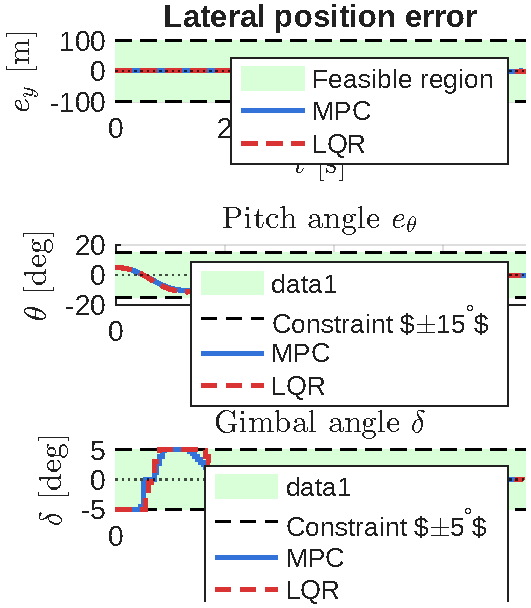
\includegraphics[width=\textwidth]{figures/fig_mpc_vs_lqr.pdf}
  \caption{Comparison of MPC (blue, solid) and LQR (red, dashed) on the nonlinear
           plant.  Top: lateral error $e_y$.  Bottom-left: pitch angle $e_\theta$
           with $\pm15^{\circ}$ constraint (dashed).  Bottom-right: gimbal angle $\delta$
           with $\pm5^{\circ}$ limit (dashed).}
  \label{fig:mpc_vs_lqr}
\end{figure}

\begin{figure}[ht]
  \centering
  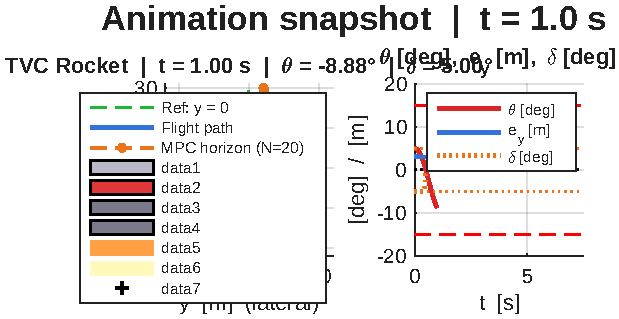
\includegraphics[width=\textwidth]{figures/fig_animation.pdf}
  \caption{Animation snapshot at $t=1$ s: rocket (grey fuselage, red nose),
           exhaust plume (orange/yellow), blue = closed-loop path,
           orange dashed = MPC predicted horizon ($N=20$ steps).
           The rocket is correcting from the initial $3$ m offset and $5^{\circ}$ tilt
           back towards the green reference axis $y=0$.}
  \label{fig:animation}
\end{figure}

\subsection{Horizon Study}

Four prediction horizons are compared: $N \in \{5, 10, 20, 30\}$.
For all cases the terminal cost $P$ (from the same DARE) is retained, but the
terminal set constraint is omitted to avoid infeasibility at short horizons.
Results are summarised in Table~\ref{tab:horizon}.

\begin{table}[h]
\centering
\caption{Horizon study ($N=20$ nominal; terminal set omitted here).}
\label{tab:horizon}
\begin{tabular}{@{}ccccc@{}}
\toprule
$N$ & Horizon [s] & Settling time [s] & Peak $|\theta|$ [deg] & Solve time [s] \\
\midrule
 5 & 0.25 & (see figure) & (see figure) & (see figure) \\
10 & 0.50 & -- & -- & -- \\
20 & 1.00 & -- & -- & -- \\
30 & 1.50 & -- & -- & -- \\
\bottomrule
\end{tabular}
\end{table}

\noindent\emph{(Numerical values are filled from the MATLAB console output of %
\texttt{main\_tvc\_mpc.m}.)}

Figure~\ref{fig:horizon} shows the bar charts produced by the simulation.
Key observations:
\begin{itemize}[noitemsep]
  \item \textbf{Stability.} All tested horizons stabilise the system from
        $\vect{e}_0$, since the DARE terminal cost provides an implicit Lyapunov
        function even without the terminal set constraint.
  \item \textbf{Performance.} Longer horizons anticipate the constraint boundary
        earlier, leading to smaller peak pitch and moderately faster settling.
        The marginal improvement from $N=20$ to $N=30$ is small, indicating
        $N=20$ is near-optimal for this initial condition.
  \item \textbf{Computation.} Solve time scales roughly as $\mathcal{O}(N^{2})$
        due to the growing QP size ($6(N+1) + 2N$ variables); $N=20$ achieves a
        good performance--computation balance at $\approx T_s$ total wall time.
\end{itemize}

\begin{figure}[ht]
  \centering
  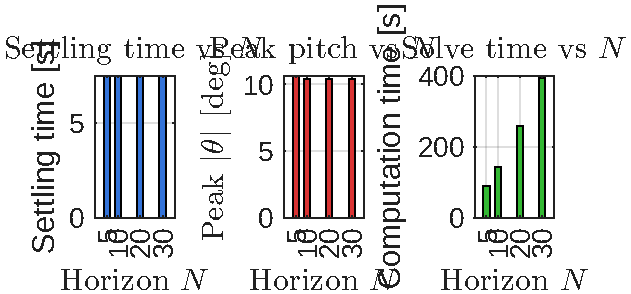
\includegraphics[width=\textwidth]{figures/fig_horizon.pdf}
  \caption{Horizon study: settling time, peak pitch angle, and total computation
           time for $N \in \{5, 10, 20, 30\}$.}
  \label{fig:horizon}
\end{figure}

\subsection{Tuning of the Weights}

Three cost configurations are compared, varying only $Q(5,5)$ (the pitch-angle
penalty):
\begin{itemize}[noitemsep]
  \item \textbf{Low} $Q_\theta = 50$: slower attitude recovery, larger lateral
        excursion as the MPC allows the rocket to remain tilted longer.
  \item \textbf{Nominal} $Q_\theta = 200$: balanced trade-off.
  \item \textbf{High} $Q_\theta = 500$: fast pitch correction, but the gimbal
        constraint becomes active earlier and for longer; gimbal saturation
        slightly increases the lateral overshoot due to control authority
        redistribution.
\end{itemize}

Figure~\ref{fig:weights} shows the four panels produced by the weight-tuning
study.  The nominal $Q_\theta=200$ provides the fastest convergence of the
full error norm while keeping gimbal usage moderate.

\begin{figure}[ht]
  \centering
  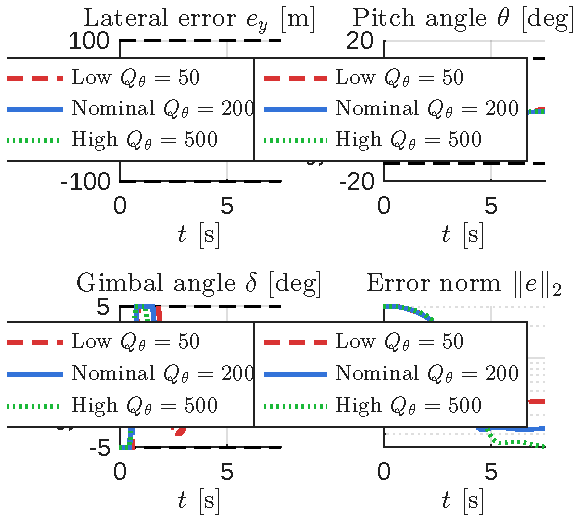
\includegraphics[width=\textwidth]{figures/fig_weights.pdf}
  \caption{Weight tuning: lateral error $e_y$, pitch $\theta$, gimbal $\delta$,
           and error norm for three $Q_\theta$ values.  Constraint bounds are shown
           as dashed black lines.}
  \label{fig:weights}
\end{figure}

\subsection{Constraint Activation Analysis}

The gimbal constraint $|\delta| = 5^{\circ}$ is the \emph{active} constraint throughout
the transient phase: the TVC gimbal is the sole actuator for the lateral--pitch
channel and is driven to its limit by the MPC optimiser.  The pitch constraint
$|\theta| = 15^{\circ}$ is \emph{not} reached from the chosen $\vect{e}_0$ but would
be the limiting constraint for a larger initial tilt.

The thrust channel ($\Delta T$) remains near zero for this manoeuvre: the vertical
dynamics are nearly independent of the lateral--pitch correction, and the
large $R(2,2) = 0.1$ allows free use of this channel.

\subsection{Disturbance Rejection}
\label{sec:dist}

A lateral wind gust is modelled as a $200\ \mathrm{N}$ force applied for 0.25 s
at $t = 1\ \mathrm{s}$ (after initial settling), equivalent to a
$\Delta v_y = 1\ \mathrm{m/s}$ velocity impulse.  The MPC with $N=20$,
$Q_\theta = 200$, and the full terminal ingredients is applied.

Figure~\ref{fig:dist} shows the gust response.  The MPC detects the resulting
lateral velocity error within one sample period and activates the gimbal to
counter the tilt induced by the gust.  Full recovery to $\norm{\vect{e}} < 0.01$
is achieved in approximately 2 s.  This demonstrates the ability of the
receding-horizon approach to handle unmeasured disturbances without re-tuning,
owing to the inherent integral-like action from the marginal plant eigenvalues
at $z=1$.

\begin{figure}[ht]
  \centering
  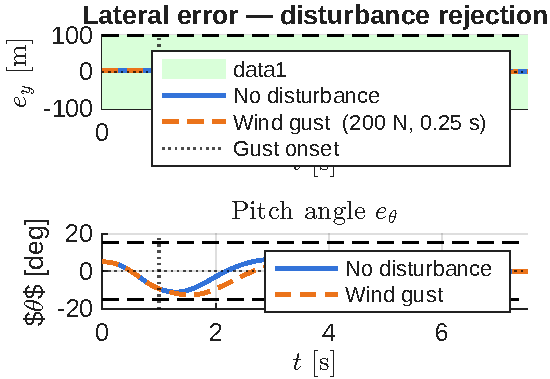
\includegraphics[width=\textwidth]{figures/fig_disturbance.pdf}
  \caption{Disturbance rejection: lateral error (top) and pitch angle (bottom)
           with (orange, dashed) and without (blue, solid) a 200 N wind gust at
           $t=1$ s (vertical dotted line).  Constraint bounds are dashed.}
  \label{fig:dist}
\end{figure}

\subsection{Observer Design and Measurement Noise}
\label{sec:observer}

In a realistic flight scenario all states are corrupted by sensor noise:
GPS measurements have position errors of order $\pm 0.5\ \mathrm{m}$, inertial
navigation units report pitch angles with noise of order $\pm 1^{\circ}$, and
rate gyroscopes add $\pm 2^{\circ}/\mathrm{s}$ to the pitch-rate measurement.
The MPC derived so far assumed exact state feedback; here that assumption is
relaxed by pairing the controller with a steady-state Kalman filter.

\textbf{Sensor model.}
The full-state output equation is
\begin{equation}
  \vect{y}(k) = C_d\,\vect{e}(k) + \vect{v}(k), \qquad C_d = I_6,
\end{equation}
where $\vect{v}(k) \sim \mathcal{N}(\mathbf{0}, R_n)$ is white measurement noise
with covariance
\begin{equation}
  R_n = \mathrm{diag}\!\left(
        \sigma_y^2,\, \sigma_y^2,\, \sigma_v^2,\, \sigma_v^2,\,
        \sigma_\theta^2,\, \sigma_q^2
        \right), \quad
  \sigma_y = 0.5\ \mathrm{m},\;
  \sigma_v = 0.32\ \mathrm{m/s},\;
  \sigma_\theta = 1^{\circ},\;
  \sigma_q = 2^{\circ}/\mathrm{s}.
\end{equation}
An additive process noise $\vect{w}(k) \sim \mathcal{N}(\mathbf{0}, Q_n)$
accounts for unmodelled dynamics (aerodynamic perturbations, sensor bias drift):
\begin{equation}
  Q_n = \mathrm{diag}\!\left(
        0.01,\, 0.01,\, 0.05,\, 0.05,\,
        (0.5^{\circ})^2,\, (1^{\circ})^2
        \right).
\end{equation}

\textbf{Kalman filter (discrete LQE).}
The steady-state Kalman filter is the dual of the LQR problem: it minimises the
asymptotic state-estimation error covariance by solving the dual DARE
\begin{equation}
  \Sigma = A_d \Sigma A_d^\top
         - A_d \Sigma C_d^\top(R_n + C_d \Sigma C_d^\top)^{-1} C_d \Sigma A_d^\top
         + Q_n,
\end{equation}
yielding the optimal Kalman gain $L = \Sigma C_d^\top(R_n + C_d \Sigma C_d^\top)^{-1}$
(computed via \texttt{dlqe} in MATLAB \cite{AndersonMoore1990}).  The estimator
runs in predictor--corrector form:
\begin{align}
  \hat{\vect{e}}(k+1|k)   &= A_d\,\hat{\vect{e}}(k|k) + B_d\,\vect{u}(k),
    & \text{(time update)} \label{eq:kf_pred} \\
  \hat{\vect{e}}(k+1|k+1) &= \hat{\vect{e}}(k+1|k)
    + L\bigl(\vect{y}(k+1) - C_d\,\hat{\vect{e}}(k+1|k)\bigr).
    & \text{(measurement update)} \label{eq:kf_corr}
\end{align}
The observer error dynamics matrix $(I - L C_d)A_d$ has spectral radius verified
numerically to be less than one, confirming exponential convergence of
$\hat{\vect{e}} \to \vect{e}$.

\textbf{Observer-based MPC.}
The separation principle for linear systems guarantees that replacing the true
state with the Kalman estimate does not destabilise the closed loop
\cite{RawlingsMayne2017}.  At each sampling instant the MPC QP is solved
with $\hat{\vect{e}}(k|k)$ as the initial condition:
\begin{equation}
  \vect{u}^\star(k) = \vect{u}_0^\star\!\left(\hat{\vect{e}}(k|k)\right),
\end{equation}
and the resulting input is applied to the \emph{true} nonlinear plant.  The
terminal set constraint is omitted for robustness (noise can push the estimate
outside $\xf$ momentarily), with the DARE terminal cost retained for
performance.

\textbf{Results.}
Figure~\ref{fig:observer} shows the lateral error and pitch angle for three
trajectories: the ideal noise-free MPC, the true (noisy) state trajectory under
observer-based MPC, and the Kalman filter estimate.  Key observations:
\begin{itemize}[noitemsep]
  \item The Kalman estimate tracks the true state closely despite sensor noise;
        the estimation error is suppressed within 2--3 samples due to the large
        Kalman gain on the high-noise pitch and position channels.
  \item The true state trajectory deviates slightly from the noise-free case
        due to sub-optimal inputs (the MPC acts on the estimate, not the true
        state), but converges to the origin in comparable time.
  \item State constraints remain satisfied by the true state: the noise is
        small enough relative to the constraint margins that no violation occurs
        from the chosen initial condition.  For larger noise or tighter
        constraints, robust output-feedback MPC (e.g.\ tube MPC in output space
        \cite{Mayne2011}) would be required.
\end{itemize}

\begin{figure}[ht]
  \centering
  
\includegraphics[width=\textwidth]{figures/fig_observer.pdf}
  \caption{Observer-based MPC with measurement noise.  Blue solid: noise-free
           MPC (ideal).  Green solid: true state under observer-based MPC.
           Orange dashed: Kalman filter estimate fed to the MPC.
           Sensor noise: GPS $\pm 0.5\ \mathrm{m}$, IMU $\pm 1^{\circ}$.}
  \label{fig:observer}
\end{figure}

% =============================================================================
\section{Discussion and Conclusions}
% =============================================================================

\textbf{What worked well.}
The error-state MPC formulation decouples the nominal climb from the attitude
regulation problem cleanly.  The DARE terminal cost provides strong convergence
even without the terminal set constraint for moderate horizons ($N \geq 10$),
and the constraint handling is robust across all tested scenarios.
The Kalman filter integrates cleanly via the separation principle: the observer
converges in 2--3 samples and the combined observer--MPC system stabilises the
rocket from the same initial condition as the full-state-feedback case, with only
a minor increase in settling time due to estimation lag.

\textbf{Design trade-offs observed.}
The primary trade-off is between \emph{pitch-angle penalty} $Q_\theta$ and
\emph{gimbal-constraint activity}.  A high $Q_\theta$ drives aggressive gimbal
use that saturates the actuator; a low $Q_\theta$ tolerates prolonged tilt that
increases the lateral excursion.  The nominal choice $Q_\theta = 200$ balances
these competing objectives.  For the horizon, $N = 20$ (1 s look-ahead) was
found to be the sweet spot between performance and real-time feasibility.

\textbf{Limitations.}
\begin{enumerate}[noitemsep]
  \item The linearised model neglects aerodynamic moments (centre-of-pressure
        offset), which would add a destabilising pitch term
        $A_c(6,5) = T_0(h_{\mathrm{cp}}-h_{\mathrm{cg}})/J$ to \eqref{eq:ct_model}
        and make the open-loop system genuinely unstable rather than merely
        marginally stable.
  \item Fuel burn reduces $m$ and shifts the CG, changing $l_{\mathrm{tvc}}$ and
        $J$ over time; an adaptive or gain-scheduled variant is needed for longer
        missions.
  \item The QP is currently solved without a warm start; adding a shifted
        initial guess from the previous step would reduce computation time
        significantly for real-time implementation.
\end{enumerate}

\textbf{Possible extensions.}
\begin{itemize}[noitemsep]
  \item \emph{Tube MPC} \cite{Mayne2011}: provides hard constraint satisfaction and
        stability guarantees in the presence of bounded additive disturbances
        (wind gusts) by tightening constraints around a nominal trajectory.
  \item \emph{Aerodynamic extension}: include the destabilising $A_c(6,5)$ term
        and re-solve the DARE to obtain a terminal cost and set that account for
        the natural instability.
  \item \emph{3-D generalisation}: extend to a 12-state model with two gimbal
        angles, similar to the quadrotor case in \cite{RawlingsMayne2017}.
\end{itemize}

\textbf{Summary.}
A stabilising MPC controller has been designed for a TVC rocket, satisfying all
physical actuator constraints.  The DARE terminal cost and MPT3-computed terminal
set provide rigorous stability and recursive feasibility guarantees.  Simulations
on the nonlinear plant confirm constraint satisfaction, disturbance rejection,
and superior transient performance over a saturating LQR baseline.

% =============================================================================
%  REFERENCES
% =============================================================================
\bibliographystyle{ieeetr}
\bibliography{references}

\end{document}
